\begin{figure}[H]
	\center

	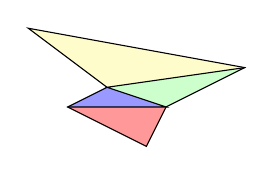
\begin{tikzpicture}[scale=1]
	
	
	% fill triangles
	\fill[red!40!white]   (0,0) -- ++(1,-0.5) -- ++(0.25,0.5) --cycle;
	\fill[blue!40!white]  (0,0) -- ++(1.25,0) --++(-0.75,0.25) --cycle;
	\fill[green!20!white]   (1.25,0) --++(-0.75,0.25) --++(1.75,0.25) --cycle;
	\fill[yellow!20!white]   (0.5,0.25) --++(1.75,0.25) --  ++(-2.75,0.5) --cycle;
	
	% outline
	\draw (0,0) -- ++(1,-0.5) -- ++(0.25,0.5)-- ++(1,0.5) -- ++(-2.75,0.5)-- ++(1,-0.75)--cycle;
	
	% this is unrobust
	\draw (0,0) -- ++(1.25,0) --++(-0.75,0.25) --++(1.75,0.25);
	
 	%\node at (1,-1) {example triangulation,};
	%\node at (1,-1.4) {$\tau$ disjunct};
	\end{tikzpicture}
		
\caption{example triangulation, $\tau$ disjunct}
\label{ch2_example_triang}

\end{figure}